\renewcommand{\thesection}{\Roman{section}}
\titleformat{\section}
{\normalfont\bfseries}{PHẦN~\thesection.}{0.4em}{}
\newcolumntype{C}[1]{>{\centering\arraybackslash}p{#1}}
\newcolumntype{L}[1]{>{\raggedright\arraybackslash}p{#1}}
\begin{tabular}{C{5cm}C{11cm}}
	\textbf{TRUNG TÂM MANABIE}& \textbf{ĐỀ ÔN TẬP KIỂM TRA GIỮA HỌC KÌ 2} \\
	\textbf{ĐỀ 03}& \textbf{Môn: VẬT LÝ}\\
	\textit{(Đề có 04 trang)}& \textit{Thời gian làm bài: 50 phút, không kể thời gian phát đề}
	
	\noindent\rule{4cm}{0.8pt} \\
\end{tabular}
\ANSMCQ{
\begin{tabular}{|C{1.2cm}|C{1.2cm}|C{1.2cm}|C{1.2cm}|C{1.2cm}|C{1.2cm}|C{1.2cm}|C{1.2cm}|C{1.2cm}|C{1.2cm}|}
	\hline
	1. C & 2. A & 3. C & 4. A & 5. C & 6. D & 7.D & 8. D & 9. A & 10. B\\
	\hline
	11. B & 12. D & 13. A & 14. A & 15. D & 16. C & 17.B & 18. C & 19. C & 20. B\\
	\hline
	21. B & 22. B & 23. A & 24. D & 25. C & 26. D & 27. C & 28. A & 29. D & 30. B\\
	\hline
\end{tabular}
}

\begin{enumerate}[label=\bfseries Câu \arabic*:]
	\item Xét tương tác của hai điện tích điểm trong một môi trường xác định. Khi lực đẩy tĩnh điện tăng hai lần thì hằng số điện môi
	\begin{mcq}(4)
		\item tăng hai lần.
		\item giảm hai lần.
		\item vẫn không đổi.
		\item giảm bốn lần.
	\end{mcq}
\hideall{
	\textbf{Đáp án C.}\\
	Hằng số điện môi không phụ thuộc vào lực tương tác điện.
}

\item Khi điện tích dịch chuyển trong điện trường đều theo chiều đường sức thì nó nhận được một công $\SI{10}{\joule}$. Khi hướng dịch chuyển tạo với chiều đường sức $\SI{60}{\degree}$ trên cùng độ dài quãng đường thì nó nhận được một công là 
\begin{mcq}(4)
	\item $\SI{5}{\joule}$.
	\item $\xsi{5\sqrt{2}}{\joule}$.
	\item $\SI{7.5}{\joule}$.
	\item $\xsi{5\sqrt{3}}{\joule}$.
\end{mcq}
\hideall{
\textbf{Đáp án A.}\\
$$\dfrac{A'}{A}=\dfrac{Fs\cos\SI{60}{\degree}}{Fs}=2\Rightarrow A'=\dfrac{A}{2}=\SI{5}{\joule}.$$
}

\item Khi độ lớn điện tích thử đặt tại một điểm tăng lên gấp đôi thì điện thế tại điểm đó
\begin{mcq}(4)
	\item giảm một nửa.
	\item tăng gấp đôi.
	\item không đổi.
	\item tăng gấp bốn.
\end{mcq}
\hideall{
\textbf{Đáp án C.}\\
Điện thế tại một điểm trong điện trường không phụ thuộc vào độ lớn điện tích thử.
}

\item Hạt nhân của một nguyên tử oxi có 8 proton và 9 neutron, số electron của nguyên tử oxi là
\begin{mcq}(4)
	\item 8.
	\item 17.
	\item 16.
	\item 9.
\end{mcq}
\hideall{
\textbf{Đáp án A.}\\
Số electrôn bằng số proton $=8$.  
}

\item Cho điện tích dịch chuyển giữa hai điểm cố định trong một điện trường đều với cường độ $\SI{150}{\volt/\meter}$  thì công của lực điện trường là $\SI{60}{\milli\joule}$. Nếu cường độ điện trường là $\SI{200}{\volt/\meter}$  thì công của lực điện trường dịch chuyển điện tích giữa hai điểm đó là
\begin{mcq}(4)
	\item $\SI{80}{\joule}$.
	\item $\SI{40}{\milli\joule}$.
	\item $\SI{80}{\milli\joule}$.
	\item $\SI{40}{\joule}$.
\end{mcq}
\hideall{
\textbf{Đáp án C.}\\
$$\dfrac{A'}{A}=\dfrac{qE'd}{qEd}=\dfrac{4}{3}\Rightarrow A'=\dfrac{4}{3}A=\SI{80}{\milli\joule}.$$
}

\item Hai điện tích điểm cùng độ lớn điện tích $\SI{E-6}{\coulomb}$  đặt trong chân không, để tương tác nhau bằng lực có độ lớn $\SI{E-3}{\newton}$  thì chúng phải đặt cách nhau
\begin{mcq}(4)
	\item $\SI{300}{\meter}$.
	\item $\SI{9}{\meter}$.
	\item $\SI{900}{\meter}$.
	\item $\SI{3}{\meter}$.
\end{mcq}
\hideall{
\textbf{Đáp án D.}\\
Ta có $F=\dfrac{kq^2}{r^2}\Rightarrow r=\left|q\right|\sqrt{\dfrac{k}{F}}=\SI{3}{\meter}.$
}

\item Đặt một điện tích thử $\SI{1}{\micro\coulomb}$  tại một điểm, nó chịu một lực điện $\SI{1}{\milli\newton}$  có hướng từ trái sang phải. Cường độ điện trường có độ lớn và hướng là
\begin{mcq}(2)
	\item $\SI{1}{\volt/\meter}$, từ trái sang phải.
	\item $\SI{1000}{\volt/\meter}$, từ phải sang trái.
	\item $\SI{1}{\volt/\meter}$, từ phải sang trái.
	\item $\SI{1000}{\volt/\meter}$, từ trái sang phải.
\end{mcq}
\hideall{
\textbf{Đáp án D.}\\
Do điện tích dường nên cường độ điện trường cùng chiều với lực điện và có độ lớn $E=\dfrac{F}{q}=\SI{1000}{\volt/\meter}$.
}

\item Một điện tích đặt tại điểm có cường độ điện trường $\SI{0.16}{\volt/\meter}$. Lực tác dụng lên điện tích đó bằng $\SI{2E-4}{\newton}$.  Độ lớn điện tích đó là
\begin{mcq}(4)
	\item $\SI{12.5E-6}{\micro\coulomb}$.
	\item $\SI{8E-6}{\micro\coulomb}$.
	\item $\SI{12.5}{\coulomb}$.
	\item $\SI{1.25E-3}{\coulomb}$.
\end{mcq}
\hideall{
\textbf{Đáp án D.}\\
Độ lớn điện tích đó là
$$\left|q\right|=\dfrac{F}{E}=\SI{1.25E-3}{\coulomb}.$$
}

\item Một tụ điện được tích điện bằng một hiệu thế $\SI{10}{\volt}$  thì năng lượng mà tụ tích được là $\SI{0.1}{\milli\joule}$. Nếu muốn năng lượng của tụ là $\SI{0.225}{\milli\joule}$ thì hai bản tụ phải có hiệu điện thế là
\begin{mcq}(4)
	\item $\SI{15}{\volt}$.
	\item $\SI{40}{\volt}$.
	\item $\SI{7.5}{\volt}$.
	\item $\SI{20}{\volt}$.
\end{mcq}
\hideall{
\textbf{Đáp án A.}\\
Năng lượng của tụ điện $$W=\dfrac{1}{2}CU^2$$
Do đó:
$$\dfrac{W_2}{W_1}=\dfrac{U^2_2}{U^2_1}\Rightarrow U_2=U_1\sqrt{\dfrac{W_2}{W_1}}=\SI{15}{\volt}.$$
}

\item Giữa hai bản kim loại phẳng song song cách nhau $\SI{4}{\centi\meter}$  có một hiệu điện thế không đổi $\SI{200}{\volt}$. Cường độ điện trường ở khoảng giữa hai bản kim loại là
\begin{mcq}(4)
	\item $\SI{800}{\volt/\meter}$.
	\item $\SI{5000}{\volt/\meter}$.
	\item $\SI{80}{\volt/\meter}$.
	\item $\SI{50}{\volt/\meter}$.
\end{mcq}
\hideall{
\textbf{Đáp án B.}\\
Cường độ điện trường giữa hai bản:
$$E=\dfrac{U}{d}=\SI{5000}{\volt/\meter}.$$
}

\item Khi điện tích dịch chuyển dọc theo một đường sức trong một điện trường đều, nếu quãng đường dịch chuyển tăng 2 lần thì công của lực điện trường
\begin{mcq}(4)
	\item không đổi.
	\item tăng 2 lần.
	\item giảm 2 lần.
	\item tăng 4 lần.
\end{mcq}
\hideall{
\textbf{Đáp án B.}\\
Do điện tích dịch chuyển dọc theo đường sức điện nên công của lực điện $A=qEs$, nếu quãng đường tăng hai lần thì công của lực điện tăng lên 2 lần.
}

\item Hai điện tích điểm đặt cách nhau $\SI{100}{\centi\meter}$  trong một môi trường có hằng số điện môi bằng 2 thì chúng tương tác với nhau bằng lực tĩnh điện có độ lớn $\SI{8}{\coulomb}$.  Nếu chúng được đặt cách nhau $\SI{50}{\centi\meter}$  trong một môi trường có hằng số điện môi bằng 10 thì chúng tương tác nhau bằng lực có độ lớn là
\begin{mcq}(4)
	\item $\SI{64}{\newton}$.
	\item $\SI{48}{\newton}$.
	\item $\SI{2}{\newton}$.
	\item $\SI{6.4}{\newton}$.
\end{mcq}
\hideall{
\textbf{Đáp án D.}\\
$$\begin{cases}
	F_1=\dfrac{k\left|q_1q_2\right|}{\varepsilon_1r^2_1}\\
	F_2=\dfrac{k\left|q_1q_2\right|}{\varepsilon_2r^2_2}
\end{cases}\Rightarrow \dfrac{F_2}{F_1}=\dfrac{\varepsilon_2r^2_2}{\varepsilon_1r^2_1}=\dfrac{4}{5}\Rightarrow F_2=\dfrac{4}{5}F_1=\SI{6.4}{\newton}.$$
}

\item Cường độ điện trường gây ra bởi điện tích $Q=\SI{5E-9}{\coulomb}$  tại một điểm trong chân không cách điện tích một khoảng $\SI{10}{\centi\meter}$  có độ lớn là
\begin{mcq}(4)
	\item $E=\SI{4500}{\volt/\meter}.$
	\item $E=\SI{0.225}{\volt/\meter}$.
	\item $E=\SI{2250}{\volt/\meter}$.
	\item $E=\SI{0.450}{\volt/\meter}$.
\end{mcq}
\hideall{
\textbf{Đáp án A.}\\
$$E=\dfrac{k\left|q\right|}{r^2}=\SI{4500}{\volt/\meter}.$$
}

\item Hai điểm M và N nằm trên cùng một đường sức của một điện trường đều có cường độ $E$, hiệu điện thế giữa M và N là $U_\text{MN}$, khoảng cách $\text{MN}=d$. Công thức nào sau đây \textbf{không đúng}?
\begin{mcq}(2)
	\item $E=U_\text{MN}d$.
	\item $U_\text{MN}=V_\text{M}-V_\text{N}$.
	\item $A_\text{MN}=qU_\text{MN}$.
	\item $U_\text{MN}=Ed$.
\end{mcq}
\hideall{
\textbf{Đáp án A.}\\
$$U_\text{MN}=V_\text{M}-V_\text{N}=Ed; \quad A_\text{MN}=qU_\text{MN}; \quad E=\dfrac{U_\text{MN}}{d}.$$
}

\item Hai điện tích điểm $q_1=\SI{-E-6}{\coulomb}$ và $q_2=\SI{6E-6}{\coulomb}$ đặt lần lượt tại A và B cách nhau $\SI{100}{\centi\meter}$. Điện trường tổng hợp bằng 0 tại
\begin{mcq}
	\item điện trường tổng hợp không thể bằng 0.
	\item trung điểm của AB.
	\item điểm M trên đường thẳng AB, ngoài đoạn AB, cách B một đoạn $\SI{69}{\centi\meter}$.
	\item điểm M trên đường thẳng AB, ngoài đoạn AB, cách A một đoạn $\SI{69}{\centi\meter}$.
\end{mcq}
\hideall{
\textbf{Đáp án D.}\\
 Để cường độ điện trường tại M bằng 0 thì 
 $$\begin{cases}
 	\vec{E}_1\uparrow\uparrow\vec{E}_2\\
 	E_1=E_2
 \end{cases}$$
Do $\begin{cases}
	\left|q_1\right|<\left|q_2\right|\\
	q_1q_2<0
\end{cases}$ nên $r_1<r_2$ và điểm M nằm gần A hơn.\\
Đặt $x$ là khoảng cách từ M đến A thì khi
$$E_1=E_2$$
$$\Leftrightarrow \dfrac{k\left|q_1\right|}{x^2}=\dfrac{k\left|q_2\right|}{\left(AB+x\right)^2}\Rightarrow x=\SI{68.9}{\centi\meter}.$$
}

\item Trong một điện trường đều, nếu trên một đường sức, giữa hai điểm cách nhau $\SI{5}{\centi\meter}$ có hiệu điện thế $\SI{10}{\volt}$, giữa hai điểm cách nhau $\SI{10}{\centi\meter}$ có hiệu điện thế là
\begin{mcq}(4)
	\item $\SI{10}{\volt}$.
	\item $\SI{15}{\volt}$.
	\item $\SI{20}{\volt}$.
	\item $\SI{22.5}{\volt}$.
\end{mcq}
\hideall{
\textbf{Đáp án C.}\\
$$\begin{cases}
	U_1=Ed_1\\
	U_2=Ed_2
\end{cases}
\Rightarrow \dfrac{U_2}{U_1}=\dfrac{d_2}{d_1}\Rightarrow U_2=\SI{20}{\volt}.$$
}

\item Một điện tích $q=\SI{E-8}{\coulomb}$ đặt trong điện trường của một điện tích điểm $Q$ thì chịu tác dụng lực $F=\SI{3}{\milli\newton}$. Biết rằng hai điện tích đặt cách nhau $r=\SI{30}{\centi\meter}$ trong chân không. Độ lớn của điện tích $Q$ là
\begin{mcq}(4)
	\item $\SI{2}{\micro\coulomb}$.
	\item $\SI{3}{\micro\coulomb}$.
	\item $\SI{4}{\micro\coulomb}$.
	\item $\SI{5}{\micro\coulomb}$.
\end{mcq}
\hideall{
\textbf{Đáp án B.}\\
$$F=qE\Rightarrow E=\dfrac{F}{q}=\SI{3E5}{\volt/\meter}$$
$$\Rightarrow E=\dfrac{k\left|Q\right|}{r^2}\Rightarrow Q=\dfrac{Er^2}{k}=\SI{3}{\micro\coulomb}.$$
}

\item Hai điện tích điểm nằm yên trong chân không tương tác với nhau bằng một lực $F$. Thay đổi các điện tích thì lực tương tác đổi chiều nhưng độ lớn không đổi. Hỏi các yếu tố trên thay đổi như thế nào?
\begin{mcq}(2)
	\item Tăng giảm sao cho $q_1+q_2$ không đổi.
	\item Tăng gấp đôi $q_1$, giảm 2 lần $q_2$.
	\item Đổi dấu $q_1$, không thay đổi $q_2$.
	\item đổi dấu $q_1$ và $q_2$.
	
\end{mcq}
\hideall{
\textbf{Đáp án C.}
}

\item Công của lực điện trường dịch chuyển một điện tích $\SI{10}{\milli\coulomb}$ song song với các đường sức trong một điện trường đều với quãng đường $\SI{10}{\centi\meter}$ là $\SI{1}{\joule}$. Độ lớn cường độ điện trường đó là
\begin{mcq}(4)
	\item $\SI{10000}{\volt/\meter}$.
	\item $\SI{100}{\volt/\meter}$.
	\item $\SI{1000}{\volt/\meter}$.
	\item $\SI{1}{\volt/\meter}$.
\end{mcq}
\hideall{
\textbf{Đáp án C.}\\
$$E=\dfrac{A}{\left|q\right|d}=\SI{E3}{\volt/\meter}.$$
}

\item Nếu hiệu điện thế giữa hai bản tụ tăng 2 lần (nhưng không vượt quá định mức) thì điện tích của tụ sẽ
\begin{mcq}(4)
	\item không đổi.
	\item tăng 2 lần.
	\item giảm 2 lần.
	\item tăng 4 lần.
\end{mcq}
\hideall{
\textbf{Đáp án B.}\\
$$\dfrac{Q'}{Q}=\dfrac{CU'}{CU}=2\Rightarrow Q'=2Q.$$
}

\item Đặt vào hai đầu tụ một hiệu điện thế $\SI{10}{\volt}$ thì tụ tích được một điện lượng $\SI{20E-9}{\coulomb}$. Điện dung của tụ là
\begin{mcq}(4)
	\item $\SI{2}{\milli\farad}$.
	\item $\SI{2}{\nano\farad}$.
	\item $\SI{2}{\farad}$.
	\item $\SI{2}{\micro\farad}$.
\end{mcq}
\hideall{
\textbf{Đáp án B.}\\
Điện dung của tụ điện $$C=\dfrac{Q}{U}=\SI{2}{\nano\farad}.$$
}

\item Cho 3 quả cầu kim loại  tích điện lần lượt $\SI{3}{\coulomb}$, $\SI{-7}{\coulomb}$ và $\SI{-4}{\coulomb}$. Khi cho chúng được tiếp xúc với nhau thì điện tích của hệ là
\begin{mcq}(4)
	\item $\SI{14}{\coulomb}$.
	\item $\SI{-8}{\coulomb}$.
	\item $\SI{-11}{\coulomb}$.
	\item $\SI{3}{\coulomb}$.
\end{mcq}
\hideall{
\textbf{Đáp án B.}\\
Điện tích của hệ:
$$Q=q_1+q_2+q_3=\SI{-8}{\coulomb}.$$
}

\item Phát biểu nào sau đây là \textbf{không đúng}?
\begin{mcq}
	\item Điện phổ của điện trường gây ra bởi một điện tích điểm là những đường thẳng song song.
	\item Các đường sức của điện trường đều là các đường thẳng song song và cách đều nhau.
	\item Điện phổ cho ta hình ảnh về hình dạng của đường sức điện.
	\item Điện phổ cho ta biết sự phân bố của các đường sức điện.
\end{mcq}
\hideall{
\textbf{Đáp án A.}\\
Đường sức điện của một điện tích điểm có dạng như hình vẽ
\begin{center}
	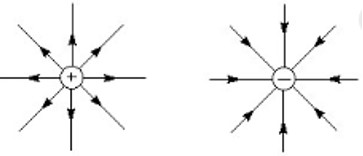
\includegraphics[width=0.3\linewidth]{../figs/PH11-MidSem2-03-1}
\end{center}
}

\item Một electron bay từ điểm M đến điểm N trong một điện trường, giữa hai điểm có hiệu điện thế $U_\text{MN}=\SI{100}{\volt}$. Công mà lực điện trường thực hiện là
\begin{mcq}(4)
	\item $\SI{100}{\electronvolt}$.
	\item $\SI{-1.6E-19}{\joule}$.
	\item $\SI{1.6E-19}{\joule}$.
	\item $\SI{-100}{\electronvolt}$.
\end{mcq}
\hideall{
\textbf{Đáp án D.}\\
Công của lực điện $$A_\text{MN}=qU_\text{MN}=\SI{-100}{\electronvolt}.$$
}

\item Hai điện tích điểm đặt trong chân không, cách nhau một đoạn $R=\SI{20}{\centi\meter}$. Lực tương tác tĩnh điện giữa chúng là $F$. Khi đặt trong dầu, ở cùng khoảng cách, lực tương tác tĩnh điện giữa chúng giảm 4 lần. Hỏi khi đặt trong dầu, khoảng cách giữa các điện tích phải là bao nhiêu để lực tương tác tĩnh điện giữa chúng cũng là $F$?
\begin{mcq}(4)
	\item $\SI{15}{\centi\meter}$.
	\item $\SI{40}{\centi\meter}$.
	\item $\SI{10}{\centi\meter}$.
	\item $\SI{12}{\centi\meter}$.
\end{mcq}
\hideall{
\textbf{Đáp án C.}\\
$$F=\dfrac{k\left|q_1q_2\right|}{r^2}; \quad F_1=\dfrac{k\left|q_1q_2\right|}{\varepsilon r^2}=\dfrac{F}{\varepsilon}=\dfrac{F}{4}\Rightarrow \varepsilon =4.$$
$$F=F''\Rightarrow \dfrac{k\left|q_1q_2\right|}{r^2}=\dfrac{k\left|q_1q_2\right|}{\varepsilon r'^2}\Rightarrow r^2=\varepsilon r'^2\Rightarrow r=2r'\Rightarrow r'=\SI{10}{\centi\meter}.$$
}


\item Hai quả cầu nhỏ mang điện tích $q_1=\SI{4}{\nano\coulomb}$, $q_2=\SI{-4}{\nano\coulomb}$ được treo ở đầu hai sợi dây cách điện dài bằng nhau trong không khí tại hai điểm treo M, N cách nhau $\SI{2}{\centi\meter}$ ở cùng một độ cao. Khi hệ cân bằng, hai dây treo lệch khỏi phương thẳng đứng, muốn đưa các dây treo về vị trí phương thẳng đứng thì phải tạo một điện trường đều $\vec{E}$ có hướng như thế nào và có độ lớn bao nhiêu?
\begin{mcq}
	\item Nằm ngang hướng từ M sang N và có độ lớn $E=\SI{9E4}{\volt/\meter}$.
	\item Nằm ngang hướng từ M sang N và có độ lớn $E=\SI{4.5E4}{\volt/\meter}$.
	\item Nằm ngang hướng từ N sang M và có độ lớn $E=\SI{4.5E4}{\volt/\meter}$.
	\item Nằm ngang hướng từ N sang M và có độ lớn $E=\SI{9E4}{\volt/\meter}$.
\end{mcq}
\hideall{
\textbf{Đáp án D.}\\
\begin{center}
	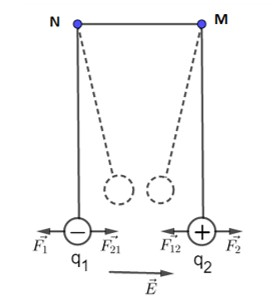
\includegraphics[width=0.4\linewidth]{../figs/PH11-MidSem2-03-2}
\end{center}
Để dây treo cân bằng
$$\left|q_1\right|E=\dfrac{k\left|q_1q_2\right|}{r^2}\Leftrightarrow E=\dfrac{k\left|q_1\right|}{r^2}=\SI{9000}{\volt/\meter}.$$
Lực tương tác giữa hai điện tích phải cùng phương ngược chiều với lực điện do điện trường đều gây ra. \\
Lực tương tác giữa hai điện tích hướng vào trong thì lực điện do điện trường gây ra phải hướng ra $\Rightarrow$ hướng nằm ngang chiều N đến M. 
}

\item Hai tụ điện có điện dung $C_1=2C_2$ mắc nối tiếp vào nguồn điện có hiệu điện thế $U$ thì hiệu điện thế của hai tụ có liên hệ là
\begin{mcq}(4)
	\item $U_2=3U_1$.
	\item $U_1=2U_2$.
	\item $U_2=2U_1$.
	\item $U_1=3U_2$.
\end{mcq}
\hideall{
\textbf{Đáp án C.}\\
Mắc nối tiếp hai tụ vào nguồn thì $$Q_1=Q_2\Rightarrow C_1U_1=C_2U_2\Leftrightarrow 2C_2U_1=C_2U_2\Rightarrow U_2=2U_1.$$
}

\item Một điện tích điểm $Q$ đặt trong không khí. Gọi $\vec{E}_\text{A}$, $\vec{E}_\text{B}$ là cường độ điện trường tại A và B do $Q$ gây ra, $r$ là khoảng cách từ A và $Q$. Để $\vec{E}_\text{A}$ có phương vuông góc với $\vec{E}_\text{B}$ và $E_\text{A}=E_\text{B}$ thì khoảng cách giữa A và B là
\begin{mcq}(4)
	\item $\sqrt{2}r$.
	\item $\sqrt{3}r$.
	\item $r$.
	\item $2r$.
\end{mcq}
\hideall{
\textbf{Đáp án A.}\\
$$\begin{cases}
	E_\text{A}=E_\text{B}\\
	\vec{E}_\text{A}=\vec{E}_\text{B}
\end{cases}\Rightarrow \begin{cases}
\text{QA}=\text{QB}=r\\
\text{QA}\bot\text{QB}
\end{cases}\Rightarrow \text{AB}=\sqrt{2}r.$$
}

\item Hai quả cầu nhỏ giống nhau có cùng khối lượng $m=\SI{0.1}{\gram}$, mang cùng điện tích $q=\SI{E-8}{\coulomb}$ được treo vào cùng một điểm bằng sợi dây mảnh trong không khí. Khoảng cách giữa hai quả cầu là $\SI{3}{\centi\meter}$. Lấy $g=\SI{10}{\meter/\second^2}$. Góc lệch của dây treo so với phương thẳng đứng là
\begin{mcq}(4)
	\item $\alpha=\SI{34}{\degree}$.
	\item $\alpha=\SI{60}{\degree}$.
	\item $\alpha=\SI{30}{\degree}$.
	\item $\alpha=\SI{45}{\degree}$.
\end{mcq}
\hideall{
\textbf{Đáp án D.}\\
\begin{center}
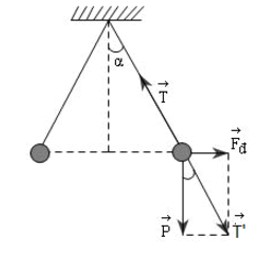
\includegraphics[width=0.3\linewidth]{../figs/PH11-MidSem2-03-3}
\end{center}
Ta có
$$\begin{cases}
	F_\text{đ}=\dfrac{k\left|q_1q_2\right|}{r^2}=\SI{E-3}{\newton}\\
	P=mg=\SI{E-3}{\newton}
\end{cases}
$$
Quả cầu cân bằng nên $$\vec{F}_\text{đ}+\vec{P}+\vec{T}=\vec{0}.$$
$$\Rightarrow \tan\alpha=\dfrac{F_\text{đ}}{P}=1\Rightarrow \alpha=\SI{45}{\degree}.$$
}

\item Một bộ gồm ba tụ điện ghép song song $C_1=C_2=\dfrac{1}{2}C_3$. Khi được tích điện bằng nguồn có hiệu điện thế $\SI{45}{\volt}$ thì điện tích của bộ tụ điện bằng $\SI{18E-4}{\coulomb}$. Điện dung của các tụ điện là
\begin{mcq}(2)
	\item $C_1=C_2=\SI{5}{\micro\farad}$, $C_3=\SI{10}{\micro\farad}$.
	\item $C_1=C_2=\SI{10}{\micro\farad}$, $C_3=\SI{20}{\micro\farad}$.
	\item $C_1=C_2=\SI{20}{\micro\farad}$, $C_3=\SI{10}{\micro\farad}$.
	\item $C_1=C_2=\SI{20}{\micro\farad}$, $C_3=\SI{40}{\micro\farad}$.
\end{mcq}
\hideall{
\textbf{Đáp án B.}\\
Điện dung của bộ tụ điện:
$$C=\dfrac{Q_b}{U}=\SI{4E-5}{\farad}.$$
Bộ tụ ghép song song 
$$\begin{cases}
	C_b=C_1+C_2+C_3=4C_1\Rightarrow C_1=\dfrac{C_b}{4}=\SI{10}{\micro\farad}\\
	C_3=2C_1=\SI{20}{\micro\farad}
\end{cases}.$$
}
\end{enumerate}
	\begin{center}
		\textbf{--- HẾT ---}
	\end{center}
